


\chapter{%State-space Covariates
%Modeling Spatial Variation in Density Using State-Space Covariates
Modeling Spatial Variation in Density
}
\markboth{Spatial Variation in Density}{}
\label{chapt.state-space}

\vspace{0.3cm}

\begin{comment} ok this is a minor tech mpoint for now: but this is introduced as a ``point process''
but what is being decribed here is a REALiZATION of a point process. Lets clarify this in the final
draft
\end{comment}
Underlying all spatial capture recapture models is a point process
model describing the distribution of individual activity
centers (${\bf s}_i$) within the state space ($\cal{S}$). So far we have focused our
attention on the homogeneous binomial point process,
${\bf s}_i \sim \mbox{Unif}({\cal S}), i=1,2,\dots,N$, where $N$ is the
size of the population. This is a model of
``spatial-randomness''\footnote{The phrase ``complete
  spatial-randomness'' is reserved for the homogeneous Poisson point
  process}
because the intensity of the
activity centers is constant across the study area and the activity
centers are distributed independently of each other.

The spatial-randomness assumption is often viewed as restrictive
because ecological processes such as
territoriality and habitat selection can result in non-random
distributions of organisms. We have argued, however, that this
assumption is less restrictive than may be recognized because the
homogeneous point process actually allows for infinite
possible configurations of activity centers. Furthermore, given enough data,
the uniform prior will have very little influence on the estimated
locations of activity centers. Nonetheless, the homogeneous point
process model does not allow one to model population density using
covariates---a central objective of much ecological research.
For example, a homogeneous point process model
may result in a density surface map indicating that individuals were
more abundant in one habitat than another, but it does not do so
explicitly. A more direct approach would be to model density using
covariates as is done in generalized linear models (GLMs)
\citep{mccullagh_nelder:1989}. % where a
%link function is used to connect the intensity parameter to the linear
%predictor.

In this chapter we present a method
for fitting inhomogeneous binomial point process models using
covariates in much the same way as is done with GLMs. The
covariates we consider differ
from those covered in previous chapters, which were typically
attributes of the animal ({\it e.g.} sex or age) or the trap ({\it
  e.g.} baited or not) and were used to model movement or encounter
rate. In contrast, here we wish to
model covariates that are defined for all points in
$\cal{S}$, which we will refer to as
state-space covariates or density covariates. These may
include continuous covariates such as elevation, or discrete
covariates such as habitat type.

\citet{borchers_efford:2008} were the first to propose an
inhomogeneous point process model for SCR models, and our approach is
similar to theirs with the exception that we will use a binomial
rather than a Poisson model because the binomial model is
easily integrated into our MCMC algorithm %data augmentation scheme
and is consistent
with the objective of determining how a {\it fixed} number of activity
centers are distributed with respect to covariates.

The method we use to accommodate inhomogeneous binomial point process
models within our MCMC algorithm is simple---we
replace the uniform prior with a prior describing the
distribution of the $N$ activity centers conditional on the
covariates. Development of this prior, which does not have a
standard form, is a central component of this chapter. First we %will
begin with a review of homogeneous point process models.


\section{Homogeneous point process revisited}

The homogeneous Poisson point process is \emph{the} model of ``complete
spatial randomness'' and is often used in ecology as a null model
to test for departures from randomness
\citep{diggle:2003,illian_etal:2008}. Given its central role in the
analysis of point processes, it is helpful to compare it with
the binomial model that we use in our SCR models. The
primary descriptor of the homogeneous point process model is the
``intensity'' parameter, $\mu$ which describes the expected number
% start with \mu(x)???? Or, wait for inhomogeneous case?
of points in an infinitesimally small area. The intensity
parameter can also be used to determine the expected number of points
in any region $B$ of the state-space $\cal{S}$. To denote this, we say
that the expected number of points in region $B \in \cal{S}$ is
$\mathbb{E}[n(B)] = A(B)\mu$ where $A(B)$ is the area of region $B$.  In words,
the expected number of points in $B$ is simply the area of $B$
multiplied by the intensity parameter. One property
of the Poisson model is that if we divide the entire state-space into $K$
%$k=1,\dots,K$
disjunct regions, the vector of counts $\{ n(B_k): k=1,\dots,K \}$ are
independent and identically distributed, ({\it i.i.d.}). This is one
of the distinctions between the Poisson model and the binomial model,
for which the counts $\{n(B_k)\}$ are not {\it i.i.d.}, as we will explain
shortly.

The two models also differ in how they regard the number of points
$N$. %This difference is also related to another distinction
%between the two models, namely that
The binomial model conditions on $N$, \textit{i.e.}, $N$ is fixed; whereas under
the Poisson model $N$ is random. Here is some simple \R~code to
illustrate this point.

\begin{center} % doesn't work
\begin{verbatim}
mu <- 4                            # intensity
Np <- rpois(1, mu)                 # Np is random
PPP <- cbind(runif(Np), runif(Np)) # Poisson point process

Nb <- 4                            # Nb is fixed
BPP <- cbind(runif(Nb), runif(Nb)) # Binomial point process
\end{verbatim}
\end{center}

Note that in both models, the $N$ points are independent
of one another and distributed uniformly
throughout $\mathcal{S}$. Thus, the intensity at any point $x \in
\cal{S}$ is $\mu = 1 / A(\mathcal{S})$ where $A(\mathcal{S})$ denotes
the area of the state-space. In the \R~code above, the area of the
state-space is 1 unit, and thus the intensity is $\mu = 1/1$.

Although the Poisson model is typically described in terms of $\mu$,
the binomial model is not; rather, it
is more common to consider a discrete state-space, such as a grid with
with $K$ pixels. Under the binomial model, the number of points in
each region is $n(B_k) \sim Bin(N, p_k)$
where $p_k = A(B)/A(\cal{S})$, \emph{i.e.} $p_k$ is simply the proportion of
the state-space area in $B_k$. This discrete space representation of
the binomial point process is shown in Fig.~\ref{ch9.fig.homo}. The
state-space in this case is the unit square, and thus the probability of a
point falling in each of the 25 disjunct regions is $p_k = 1/25$ and
the expected counts are simply $\mathbb{E}(n(B_k)) = Np_k$. In
the figure $N=50$, and consequently, we would expect 2 points per pixel, which
happens to be the empirical mean of the data in
Fig.~\ref{ch9.fig.homo}. Note also that these counts are not
independent realizations from a binomial distribution since $\sum_{k=1}^K
n(B_k) = N$. Instead, the model for the entire vector
is ${\bf n(B)} \sim \mbox{Multinom}(N, {\bm{\pi}} = \{p_1, p_2, \dots,
p_K \})$ \citep{illian_etal:2008}. The dependence among counts has virtually
no practical consequence when the number of pixels is large. For
example, if there are 100 pixels, the number of points in one pixels
carries very little about the expected number of points in another
pixel. However, if there are only 2 pixels, then clearly the number of
points in one pixel allows one to determine how many points will occur in the
remaining pixel. To gain familiarity with the multinomial distribution
and the discrete representation of space, use the \verb+rmultinom+
function in \R~to simulate counts similar to those shown in
Fig.~\ref{ch9.fig.homo}, for example using commands
such as:
\begin{verbatim}
n.Bk <- rmultinom(1, size=50, prob=rep(1/25, 25))
matrix(n.Bk, 5, 5)
\end{verbatim}


\begin{figure}
\centering
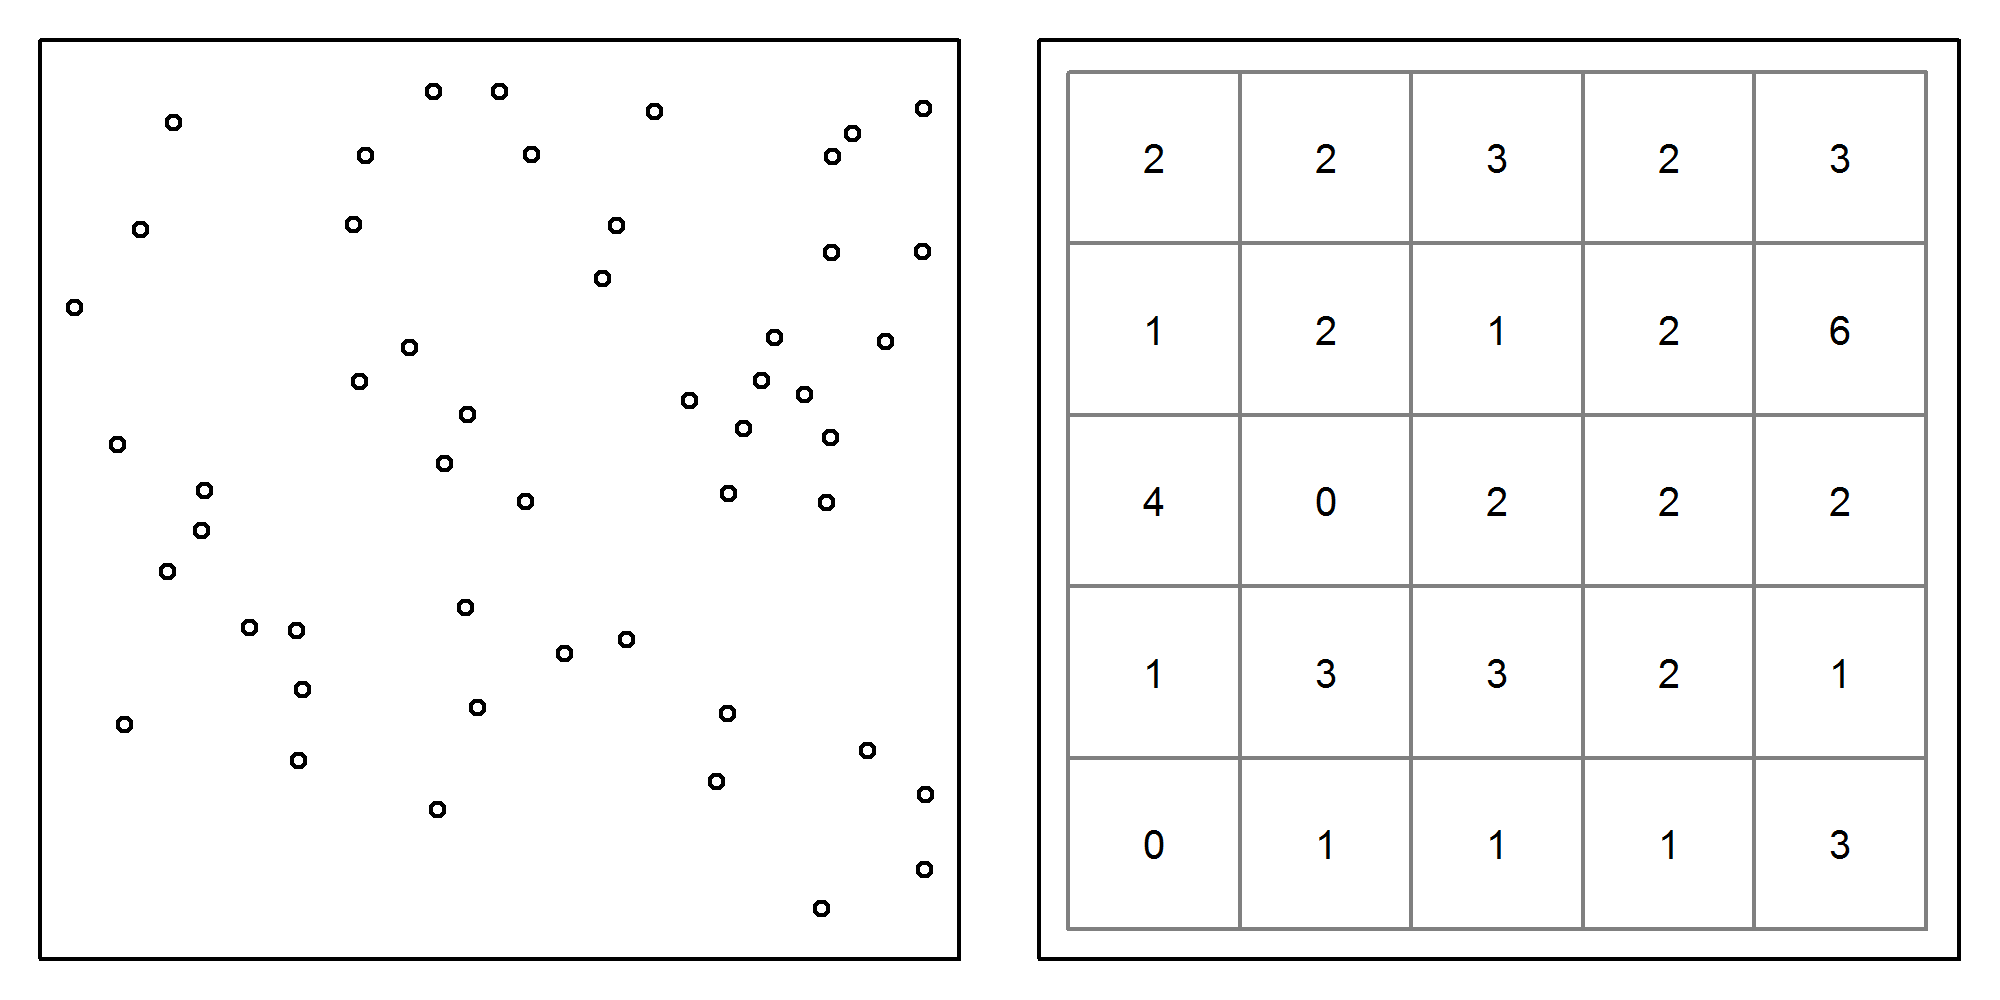
\includegraphics[width=5in,height=2.5in]{Ch11/figs/homoPlots}
\label{ch9.fig.homo}
\caption{Homogeneous binomial point process with $N$=50 points
  represented in continuous and discrete space.}
\end{figure}


The discrete space representation of the binomial point process is of
practical importance when fitting SCR models because spatial covariates
are almost always represented in a discrete-space format called
``rasters'' in GIS-speak. In such cases, we often need to change our
definition of the prior for an activity center from ${\bf s}_i \sim
\mbox{Unif}(\cal{S})$ to ${\bf s}_i \sim \mbox{Multin}(1, \mathbf{\pi})$. In the
latter case, the activity center is simply defined as an integer
representing pixel ``id''. Note also that the multinomial distribution
with an index of 1 (\emph{i.e.} \verb+size=1+ in \verb+rmultinom+)
is referred to as the categorical distribution,
which we will frequently use in the \verb+BUGS+ language.



\section{Inhomogeneous binomial point process}

As with the homogeneous model, the inhomogeneous binomial point process
model is developed conditional on $N$. The primary distinction is that
the uniform distribution is replaced with another distribution
allowing for the intensity parameter to vary spatially. To arrive at
this new distribution, replace the scalar intensity parameter $\mu$
with the function $\mu(x, {\bm \beta})$, where $\bm \beta$ is a
vector of coefficients describing the effects of
spatially-referenced covariates on the point process intensity.
Since an intensity must be strictly
positive, it is natural to model $\mu(x, \beta)$ using the log-link.
\[
\log(\mu(x, \beta)) = \sum_{j=1}^J \beta_j v_j(x), \quad  x \in \cal{S}
\]
where $\beta_j$ is the regression coefficient for covariate
$v_j(x)$. To be clear, $v(x)$ is the value of any covariate, such as
habitat type or elevation, defined at all points in  the state-space.
This equation should look
familiar because it is the standard linear predictor used in log-linear
GLMs. Note, however, that we have no need
for an intercept because it would be confounded with
$N$ (see Chapt. \ref{chapt.hscr}). This should be intuitive since an intercept would
represent the expected value of $N$ when $\beta=0$, but we already
have a parameter in the model for expected abundance, namely $\mathbb{E}[N] =
\psi M$\footnote{Remember, $M$ is the size of the augmented population, and
$\psi$ is the probability that a member of $M$ is an actual
constituent of the population (Chapt. ~\ref{chapt.scr0}).}. Thus an intercept would be
redundant, and without it we are still able to achieve our goal of
describing the distribution of $N$ activity centers as a function of
spatial covariates.

Now that we have a model of the intensity parameter $\mu(x)$,
we need to develop the associated probability density function to use
in place of the uniform prior. Remembering that
the integral of a pdf must be unity, we can create a pdf by dividing
$\mu(x)$ by a normalizing constant, which in this case is the integral
of $\mu(x)$ evaluated over the entire
state-space. \begin{comment}
this is the conditional probability distribution of location -- i.e., conditional on their being a point in x, this
is the probability distribution of its location. I think we need to use the term ``conditional probability distribution''
and maybe a concise coherent justification can be copied out of Illian at a later date. we can also contemplate
this later and resolve things
\end{comment}
The
probability density function is therefore
\begin{equation}
f(x, \beta) = \frac{\mu(x, \beta)}{\int_{x \in \mathcal{S}} \mu(x, \beta)\, \mathrm{d}x}
\label{eq.pdf.ipp}
\end{equation}
Substituting this distribution for the
uniform prior allows us to fit inhomogeneous binomial point process
models to spatial capture-recapture data. We can also use this
distribution to obtain the expected number of individuals in any given
region. Specifically, the proportion of $N$ expected to occur in any
region $B$ when heterogeneity in density is present is $p(B) = \int_B
f(x, \beta)\, \mathrm{d}x$. These are
also the multinomial cell probabilities if the regions are
disjoint and compose the entire state-space. We provide an example in
the next section, and in Fig.\ref{ch9.fig.hetero}.

As a practical matter, note that the integral in the
denominator of $f(x, \beta)$ is evaluated over space, and since we always regard
space as two-dimensional, this is a two-dimensional integral that can
be approximated using the methods discussed in
Chapter~\ref{chapt.poisson-mn}. These methods include
Monte Carlo integration, Gaussian quadrature, etc... Alternatively, if
our state-space covariates are in raster format, \emph{i.e} they are
in discrete space, the integral can be replaced with a sum over
all pixels,
\begin{equation}
f(x, \beta) = \frac{\mu(x, \beta)}{\sum_{x \in \mathcal{S}} \mu(x, \beta)\, \mathrm{d}x}
\label{eq.pdf.dipp.d}
\end{equation}
which is much more efficient computationally.

We now have all the tools needed to fit inhomogeneous point process
(IPP) models. If we refer to the distribution for the
inhomogeneous point process as ``IPP'', we can write a
hierarchical description of a SCR model with a Poisson encounter process and
a half-normal detection function as
\begin{gather*}
w_i \sim \mbox{Bern}(\psi) \\
{\bf s_i} \sim \mbox{IPP}(\mu(x,\beta)) \\
\lambda_{ij} = \lambda_0 \exp(-\|{\bf s_i} - {\bf x_{j}}\|^2/(2\sigma^2)) \\
y_{ij} \sim \mbox{Poisson}(\lambda_{ij} w_i)
\end{gather*}
The use of $\mbox{IPP}(\mu(x, \beta))$ instead of
$\mbox{Unif}(\cal{S})$ is the only difference between a homogeneous
point process model and an inhomogeneous point process model, and the
two are equivalent when $\beta=0$.

\begin{comment}
The IPP for the activity centers
results in another IPP for the observation process, $\lambda(x)$, the
expected number of captures for a trap
at point. As was true for the homogeneous model, this
intensity function is a product of the point process intensity
and the encounter rate function, $\lambda(x) = \mu(x, {\bm \beta})
\lambda_{ij}$.
\end{comment}

In the next sections we walk through a few examples, building up from
the simplest case where we actually observe the activity centers as
though they were data. In the second example, we fit our new model to simulated
data in which density is a function of a single continuous
covariate. To build upon the developments in the previous chapter, we
further consider the plausible case where a state-space covariate is also a
covariate of ecological distance. A small simulation study indicates
that both effects can be estimated. Example four shows an analysis in discrete space using
both \secr~\citep{efford:2011} and \jags~\citep{plummer:2003}. In the
last example, we model the intensity of
activity centers for a real dataset collected on jaguars
(\emph{Panthera onca}) in Argentina.

\section{Observed Point Processes}

In SCR models, the point process is not directly observed, but in
other contexts it is. Examples include the locations of disease
outbreaks, the locations of trees in a forest, or the locations of
radio-tracked animals. Indeed Eq.~\ref{eq.pdf.ipp} has been used
extensively in the radio-telemetry literature to model so-called
``resource selection functions'' \citep{manly_etal:2002,lele_keim:2006}.
When the point locations are directly observed,
estimating the parameters $\bf \beta$ is straight-forward as
demonstrated in the following example. This example also illustrates
the fundamental process that we will later embed in our MCMC algorithm
used to fit SCR models with IPP.

Suppose we knew the locations of 100 animals' activity
centers, perhaps as the result of an extensive telemetry study. To
estimate the intensity surface $\mu(x, \beta)$ underlying these
points, we need to derive the likelihood for our data under this
model. Given the probability density function $f(x, \beta)$
(Eq.~\ref{eq.pdf.ipp}) and assuming that the points are
mutually independent of one another,
the likelihood is given by the product
of $R$ such terms, where $R=100$ is the sample size in our
hypothetical example,
\emph{i.e.} the observed number of activity centers.
\[
\mathcal{L}({\bf \beta} | {\bf x}_i, \beta) = \prod_{i=1}^R f(x_i)
\]
Having defined the likelihood we could choose a prior distribution for
$\beta$ and obtain the posterior distribution of
$\bf \beta$ using Bayesian methods, or we can find the maximum likelihood
estimates (MLEs) using standard numerical methods as is demonstrated
below.

First, we simulate some data. Simulating data under an inhomogeneous point process model is often
accomplished using indirect methods such as rejection
sampling. Rejection sampling proceeds by
simulating data from a standard distribution and then accepting or
rejecting each sample using probabilities defined by the distribution
of interest. For more information, readers should consult an
accessible text such as \citet{robert_casella:2010}. In our example, we
simulate from a uniform distribution and then accept or reject using
the (scaled) probability density function $f(x, \beta)$. Note that we first define a
spatial covariate (elevation) that is a simple function of the spatial
coordinates increasing from the southwest to the northeast of our
state-space.\footnote{Such functional forms of
covariates are rarely available. Instead,  continuous spatial
covariates are more often measured on a discrete grid.}

The following \R~commands demonstrate the use of rejection sampling to
simulate an inhomogeneous point process for the covariate depicted in
Fig.~\ref{ch9.fig.hetero}. The code uses the \verb+cuhre+ function in
the {\tt R2Cuba} package to integrate the intensity function over
space \citep{hahn_etal:2011}. An alternative would be to evaluate the
integral on a fine grid of points as we have done in previous
chapters, but it is useful to gain familiarity with more efficient
integration functions in \R.

\begin{small}
\begin{verbatim}
# spatial covariate (with mean 0)
elev.fn <- function(x) x[1]+x[2]-1
# intensity function
mu <- function(x, beta) exp(beta*elev.fn(x=x))

# Simulate IPP using rejection sampling
set.seed(300225)
N <- 100
count <- 1
s <- matrix(NA, N, 2)
beta <- 2 # parameter of interest
elev.fn <- function(x) x[1]+x[2]-1
# Intensity function, mu(x,beta)
mu <- function(x, beta) exp(beta*elev.fn(x=x))
# 2-dimensional integration over space
int.mu <- R2Cuba:::cuhre(2, 1, mu, beta=beta)$value
elev.min <- elev.fn(c(0,0)) #elev.fn(cbind(0,0))
elev.max <- elev.fn(c(1,1)) #elev.fn(cbind(1,1))
Q <- max(c(exp(beta*elev.min) / int.mu,   #2d(beta),
           exp(beta*elev.max) / int.mu))   #2d(beta)))
while(count <= 100) {
  x.c <- runif(1, 0, 1); y.c <- runif(1, 0, 1)
  s.cand <- c(x.c,y.c)
  pr <- exp(beta*elev.fn(s.cand)) / int.mu #2d(beta)
  if(runif(1) < pr/Q) {
    s[count,] <- s.cand
    count <- count+1
    }
  }
\end{verbatim}
\end{small}


\begin{figure}
\centering
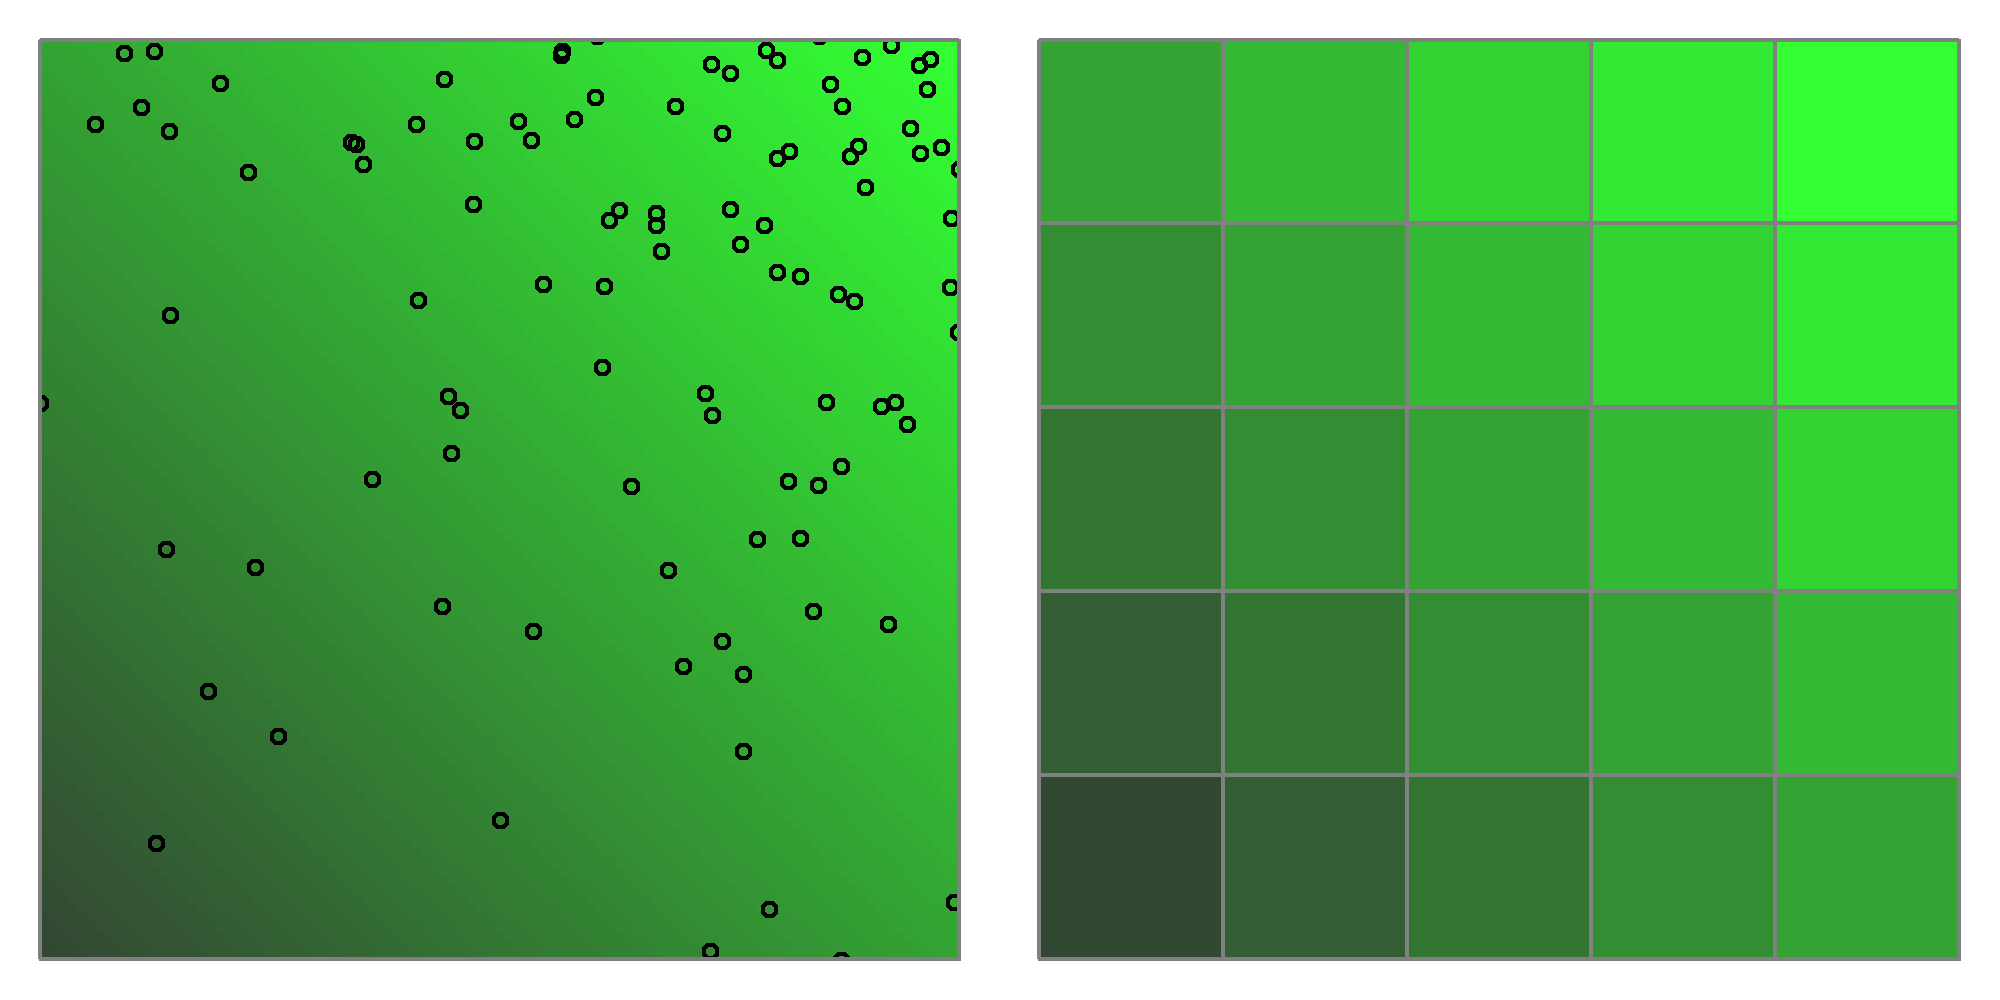
\includegraphics[width=5in,height=2.5in]{Ch11/figs/heteroPlots}
\label{ch9.fig.hetero}
\caption{An example of a spatial covariate, say elevation, and a
  realization of a inhomogeneous binomial point process with $N$=100
  and $\mu(x) = exp(\beta \mbox{elev}(x))$ where $\beta=2$.}
\end{figure}

The simulated data are shown in Fig~\ref{ch9.fig.hetero}. High elevations
are represented by light green and low elevations by dark green. The
activity centers of 100 animals are shown as
points, and it is clear that these simulated animals prefer the high
elevations.  Perhaps they are mountain goats. The underlying model describing this preference is
$\log(\mu(x)) = \exp(\beta \times elev(x))$
where $\beta=2$ is the parameter to be estimated.

Given these points, we will now estimate $\beta$ by minimizing the
negative-log-likelihood using \verb+R+'s \verb+optim+ function.

\begin{small}
\begin{verbatim}
# Negative log-likelihood
nll <- function(beta) {
    int.mu <- R2Cuba:::cuhre(2, 1, mu, beta=beta)$value
    -sum(beta*elev.fn(s) - log(int.mu))
}
starting.value <- 0
fm <- optim(starting.value, nll, method="Brent",
            lower=-5, upper=5, hessian=TRUE)
c(Est=fm$par, SE=sqrt(1/fm$hessian)) # estimates and SEs
\end{verbatim}
\end{small}


Maximizing the likelihood took a small fraction of a second, and we
obtained an estimate of $\hat{\beta}=1.99$. We could plug
this estimate into our linear model at each point in the state-space to
obtain the MLE for the intensity surface.

This example demonstrates
that if we had the data we wish we had, {\it i.e.} if we knew the
coordinates of the activity centers $\bf s$, we could easily estimate the
parameters governing the underlying point process. Unfortunately, in
SCR models, the activity centers cannot be directly observed, but
spatial re-captures provide us with the information needed to
estimate these latent parameters.

\section{Fitting inhomogeneous point process SCR models}

\subsection{Continuous space}

One of the nice things about hierarchical models is that they allow us
to break a problem up into a series of simple conditional
models. Thus,
we can simply add the methods described above into our existing MCMC
algorithm to simulate the posteriors of $\beta$ conditional on the
simulated values of $\mathbf{s}$. To demonstrate, we will continue with
the previous example. Specifically, we will overlay a grid of
traps upon the map shown in Fig.~\ref{ch9.fig.hetero}. We will then
simulate capture histories conditional upon the activity
centers. Then, we will attempt to estimate the activity center
locations as though we did not know where they were, as is the case in
real applications.

The following \R~code simulates encounter histories under a
Poisson observation model (see Chapt. \ref{chapt.poisson-mn}), which could be appropriate in camera
trapping studies or when using other methods in which animals could
be detected multiple times at a trap during a single occasion.

\begin{small}
\begin{verbatim}
# Create trap locations
xsp <- seq(-0.8, 0.8, by=0.2)
len <- length(xsp)
X <- cbind(rep(xsp, each=len), rep(xsp, times=len))

# Simulate capture histories, and augment the data
ntraps <- nrow(X)
T <- 5
y <- array(NA, c(N, ntraps, T))

nz <- 50 # augmentation
M <- nz+nrow(y)
yz <- array(0, c(M, ntraps, T))

sigma <- 0.1  # half-normal scale parameter
lam0 <- 0.5   # basal encounter rate
lam <- matrix(NA, N, ntraps)

set.seed(5588)
for(i in 1:N) {
    for(j in 1:ntraps) {
        distSq <- (s[i,1]-X[j,1])^2 + (s[i,2] - X[j,2])^2
        lam[i,j] <- exp(-distSq/(2*sigma^2)) * lam0
        y[i,j,] <- rpois(T, lam[i,j])
    }
}
yz[1:nrow(y),,] <- y # Fill
\end{verbatim}
\end{small}

Now that we have a simulated capture-recapture dataset $y$, and we have
augmented it to create the new data object $yz$, we are ready to
begin sampling from the posteriors. A commented Gibbs sampler written
in \R~is available in the accompanying \R~package \scrbook~(see
?scrIPP). There are two small parts of the
\R~code that distinguish it from previous code we have shown to
fit homogeneous point processes. First, we need to update the parameter
${\bf \beta}$ conditional on all other parameters in the model. The code to
do so is: \begin{comment} need cite to Ch 2 or 7 on MCMC for this \end{comment}

\begin{small}
\begin{verbatim}
# Denominator of f(x, beta). Integral of mu(x, beta) over space
D1 <- cuhre(2, 1, mu, lower=c(xlims[1], ylims[1]),
            upper=c(xlims[2], ylims[2]), beta=beta1)$value
# Compute the denominator again using a proposed beta1
beta1.cand <- rnorm(1, beta1, tune[3])
D1.cand <- cuhre(2, 1, mu, lower=c(xlims[1], ylims[1]),
                 upper=c(xlims[2], ylims[2]), beta=beta1.cand)$value
# Compute log(f(x))
ll.beta1 <- sum(  beta1*elev.fn.v(S) - log(D1) )
ll.beta1.cand <- sum( beta1.cand*elev.fn.v(S) - log(D1.cand) )
if(runif(1) < exp(ll.beta1.cand - ll.beta1) )  {
     beta1<-beta1.cand
}
\end{verbatim}
\end{small}
Next, we need to put the new prior on the activity centers:
\begin{comment} see Ch 7 MCMC for SCR and cite some section of that \end{comment}
\begin{small}
\begin{verbatim}
# Compute the prior for s_i and a candidate. denominator is constant
prior.S <- beta1*elev(S[i,1], S[i,2]) # - log(D1)
prior.S.cand <- beta1*elev(Scand[1] + Scand[2]) # - log(D1)
if(runif(1)< exp((ll.S.cand+prior.S.cand) - (ll.S+prior.S))) {
    S[i,] <- Scand
    lam <- lam.cand
    D[i,] <- dtmp
    }
\end{verbatim}
\end{small}

We can apply this modified sampler to our data using the
following \R~commands.
\begin{small}
\begin{verbatim}
set.seed(3434)
fm1 <- scrIPP(yz, X, M, 6000, xlims=c(0,1), ylims=c(0,1),
            tune=c(0.003, 0.08, 0.3, 0.07) )
plot(mcmc(fm1$out))
rejectionRate(mcmc(fm1$out))
\end{verbatim}
\end{small}

We obtain posterior
distributions summarized in Table~\ref{ch9.tab.simIPP}. Mixing is good, and as usual,
life is very nice when we are working with simulated data.

\begin{table}[b]
\centering
\caption{Posterior summaries from inhomogeneous point process model}
\begin{tabular}{lrrrrr}
\hline
& Mean & SD & 2.5\% & 50\% & 97.5\% \\
\hline
 $\sigma =0.10$ &   0.1026 &   0.0048 &   0.0935 &   0.1025 &   0.1123 \\
 $\lambda_0=0.50$ &   0.4419 &   0.0493 &   0.3496 &   0.4400 &   0.5390 \\
 $\psi =0.66$ &   0.6826 &   0.0554 &   0.5762 &   0.6820 &   0.7923 \\
 $\beta =2.00$ &   2.1601 &   0.3390 &   1.5193 &   2.1583 &   2.8043 \\
 $N =100$ & 102.7696 &   6.2689 &  92.0000 & 102.0000 & 117.0000 \\
\hline
\end{tabular}
\label{ch9.tab.simIPP}
\end{table}


Fitting continuous space IPP models is somewhat
difficult in \bugs~because our prior ``IPP'' is not one of the
available distributions that come with the software. It is
possible to add new distributions in \bugs, but it is somewhat
cumbersome.  \secr~allows
users to fit continuous space IPPs using polynomials of the x- and y-
coordinates, but it does not accept truly continuous covariates that
are functions of space. However, these
are not really important limitations because discrete
space versions of the IPP model are straight-forward, and virtually all spatial
covariates are, or can be, defined as such.


\subsection{Discrete space}

To fit IPPs using covariates in discrete space, \emph{i.e.} in raster
format, we follow the same steps
as outlined in Chapter~\ref{chapt.poisson-mn}---we define ${\bf s}_i$ as
pixel ID, and we use the categorical distribution as a prior. A good
example is found in \citep{mollet_etal:2012}. Here we present
an analysis of the simulated data shown in the right panel of
Fig.~\ref{ch9.fig.hetero}. The spatial covariate, let's call it
elevation again, was simulated
using using the code shown on the help page
\verb+ch9simData+ in \scrbook. The points are the number of
activity centers in each pixel, generated from a single realization of
the inhomogeneous point process model with intensity
$\mu(x) = 2 \times \mbox{elev}(x)$.
\begin{figure}
\centering
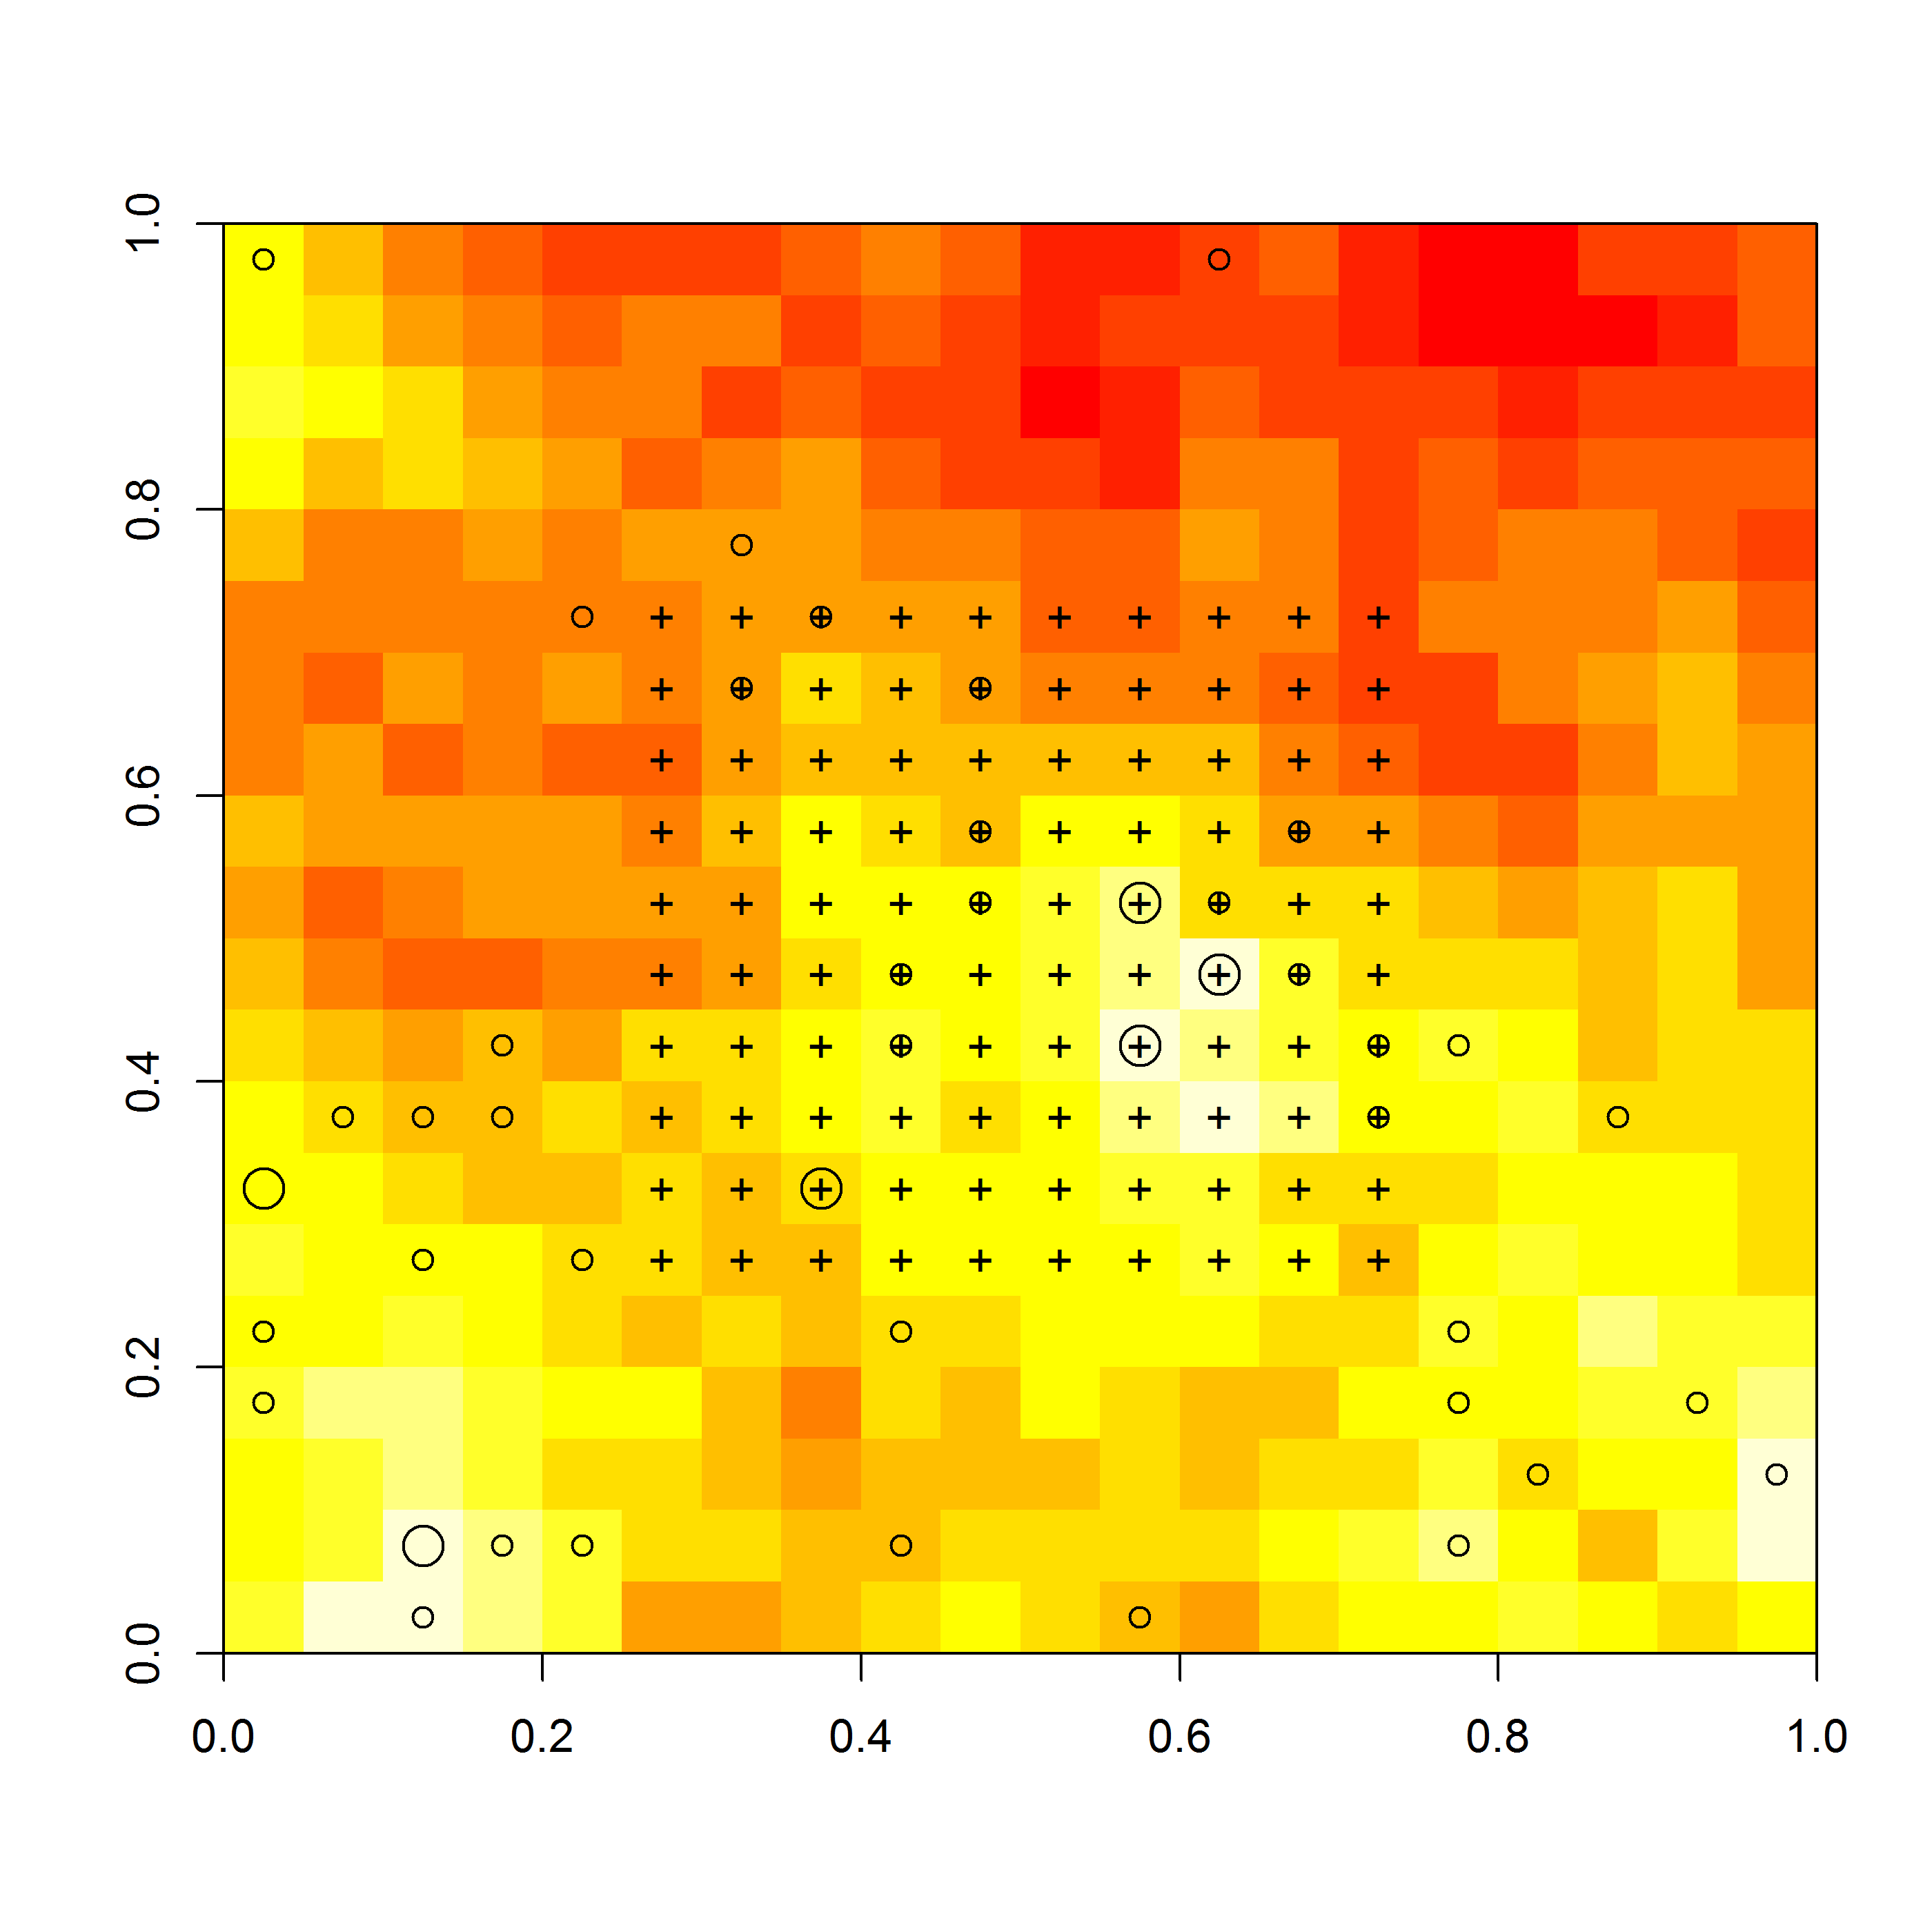
\includegraphics[width=3in,height=3in]{Ch11/figs/discrete}
\label{ch9.fig.discrete}
\caption{Simulated activity centers in discrete space. The spatial
  covariate, elevation, is highest in the lighter areas. Density of
  activity centers (circles) increases with elevation. A single
  activity center is shown as a small circle, and larger circles
  represent two activity centers in a pixel. Trap locations
  are shown as crosses.}
\end{figure}

The \bugs~code to fit an IPP model to these data is shown in
panel~\ref{ch9.panel1}.The vector \verb+probs[]+ is the prior
probability defined
by~\ref{eq.pdf.ipp.d}, which is the probability that an individual's
activity center is located at pixel $x$. \verb+Sgrid+ is the
matrix of coordinates for each pixel.

%\begin{panel}[h!]
%\centering
%\rule[0.15in]{\textwidth}{.03in}
\begin{small}
\begin{verbatim}
model{
sigma ~ dunif(0, 1)
lam0 ~ dunif(0, 5)
beta ~ dnorm(0,0.1)
psi ~ dbeta(1,1)
for(x in 1:nPix) {
  theta[x] <- exp(beta*elevation[j])
  probs[x] <- theta[j]/sum(theta[])
}
for(i in 1:M) {
  w[i] ~ dbern(psi)
  s[i] ~ dcat(probs[])
  x0g[i] <- Sgrid[s[i],1]
  y0g[i] <- Sgrid[s[i],2]
  for(j in 1:ntraps) {
    dist[i,j] <- sqrt(pow(x0g[i]-grid[j,1],2) +
                      pow(y0g[i]-grid[j,2],2))
    lambda[i,j] <- lam0*exp(-dist[i,j]*dist[i,j] /
                            (2*sigma*sigma)) * w[i]
    y[i,j] ~ dpois(lambda[i,j])
    }
  }
N <- sum(w[])
Density <- N/1 # unit square
}
\end{verbatim}
\end{small}
%\rule[0.15in]{\textwidth}{.03in}
%\caption{\bugs~code for fitting inhomogeneous point process model in
%  discrete space.}
%\label{ch9.panel1}
%\end{panel}

This model can also be fit in \secr, which refers
to the raster data as a ``habitat mask''. \R~code to
fit the models using \secr~and \jags~is available in \scrbook---see
\verb#help(ch9secrYjags)#. Results of the
comparison are shown in Table \ref{ch9:tab:secrYjags} and are
very similar as expected.
\begin{comment}
\hl{ANDY, is there any point in discussing
  the slight differences?}
  YES: If we can explain it. Could it be MC error alone?
Otherwise I guess attributing it to differences between MLE and BAyes is ok. That seems like
a reasonable thing.
\end{comment}
\begin{table}[h!]
\centering
\caption{Comparison of \secr~and \jags~results. Point estimates from
  the Bayesian analysis are posterior means. Intervals are lower and
  upper 95\% CIs.}
\begin{tabular}{llrrrr}
\hline
Software & Parameter & Estimate & SD & lower & upper \\
\hline
 secr & $N=50$ & 49.2803 & 5.7535 & 41.0087 & 64.3879 \\
      & $\beta=2$ &  2.1772 & 0.5628 &  1.0741 &  3.2804 \\
      & $\lambda_0=0.8$ &  0.9203 & 0.0764 &  0.7824 &  1.0825 \\
      & $\sigma=0.1$ &  0.0990 & 0.0038 &  0.0918 &  0.1068 \\
\hline
 JAGS & $N=50$ & 48.2072 & 5.4053 & 39.0000 & 60.0000 \\
      & $\beta=2$ &  2.1026 & 0.5323 &  1.0889 &  3.1506 \\
      & $\lambda_0=0.8$ &  0.9328 & 0.0766 &  0.7898 &  1.0921 \\
      & $\sigma=0.1$ &  0.1004 & 0.0041 &  0.0929 &  0.1089 \\
\hline
\end{tabular}
\label{ch9:tab:secrYjags}
\end{table}


\section{Ecological distance and state-space covariates}

Habitat characteristics that affect population
density could also affect home range size and movement behavior. For
example, a
species that occurs in high density in a forest may be reluctant to
venture from a forest patch into an adjacent field. Thus, even if a
trap placed in a field is located very close to an animal's activity
center, the probability of capture may be very low. In this case
forest cover is a covariate of both density and encounter probability,
and we could model it as such by combining the methods described in
this chapter and in Chapter~\ref{chapt.ecoldist}. To demonstrate, we
continue with our analysis of the data shown in
Fig~\ref{ch9.fig.hetero}. Once again, we suppose that density
increases with elevation, but this time, we also make the
assumption that home range size decreases as density increases. This
commonly-observed phenomenon can be explained by numerous factors such
as intra-specific competition \citep{sillett_etal:2004} or optimal
foraging behavior \citep{tufto_etal:1996,said_servanty:2005}. To model
this effect, we
introduce the parameter $\theta$, which determines the ``cost'' of
moving between pixels. If $\theta=0$, then the animal perceives
distance as Euclidean. If $\theta>0$, then least-cost distance (LCD)
is greater than than Euclidean distance (ED). In most cases, we would
not expect,
or should not even consider the possibility of $\theta<0$ because this
implies that LCD$<$ED, which would mean that an animal could view
1000km as 1m. In addition to the fact that this is not biologically
justifiable, it also suggests that the area of the state-space could
be infinitely large. Thus, one may want to enforce the constraint that
$\theta$ is strictly $\geq 0$. See Chapter~\ref{chapt.ecoldist} for
more details.

One may wonder if it is possible to estimate both $\beta$
and $\theta$ using standard SCR data. Currently, it is not possible to
model least-cost distance using \jags~or \secr, so we wrote our own
function, \verb+scrDED+, to fit the model using maximum likelihood. An
example analysis is provided on the help page for the function in our
\R~package \scrbook. We briefly note here that the function requires
the capture history data, the trap locations, and the raster data
formatted using the {\tt raster} package
\citep{hijmans_vanetten:2012}. The linear model for the
intensity parameter $\mu(x, \beta)$ and the least-cost distance
function $lcd(\theta)$ are specified using \R's formula interface. A
simple function call is
\begin{verbatim}
fm <- scrDED(y, traplocs=X, den.formula=~elev, dist.formula=~elev,
             rasters=elev.raster)
\end{verbatim}
To assess the possibility of estimating both $\beta$ and $\theta$, we
conducted a small simulation study, generating 500 datasets from the
model with both parameters set to 1, which corresponds to the
conditions described above. Rather incredibly, we see that it is
possible to estimate both parameters with high accuracy
(Fig~\ref{ch9.fig.sim}).

\begin{figure}
\centering
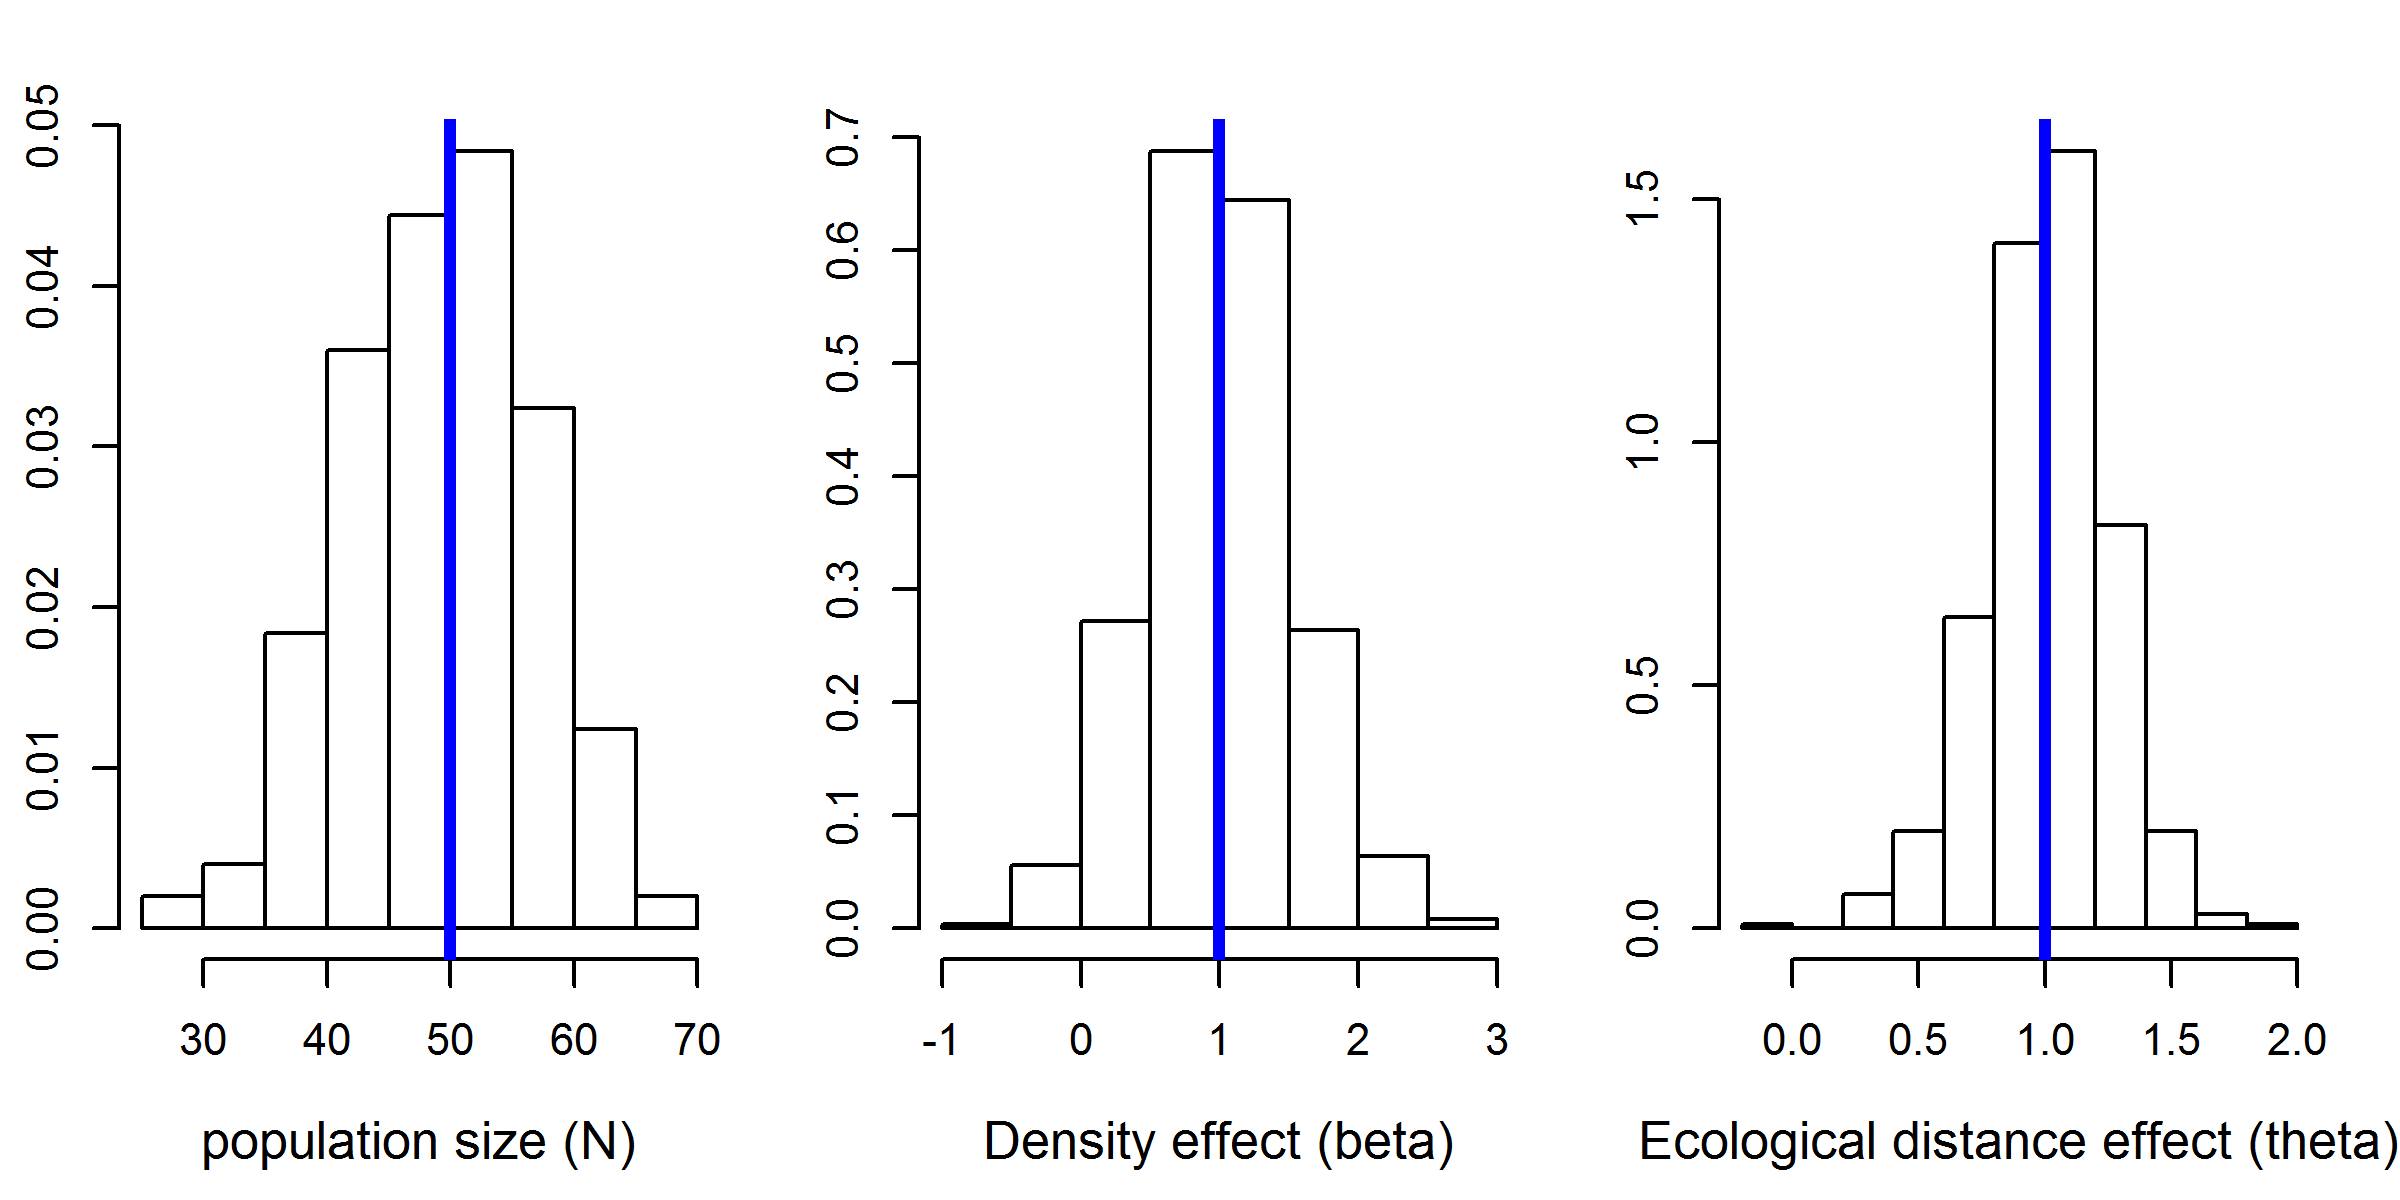
\includegraphics[width=4in,height=2in]{Ch11/figs/scrDEDsim}
\caption{Histograms of parameter estimates from 500 simulations under
  the model in which both density and ecological distance are affected
by the same covariate, elevation. The vertical lines indicate the
data-generating value.}
\label{ch9.fig.sim}
\end{figure}



\section{The jaguar data}

Estimating density of large felines has been a priority for many
conservation organizations, but no robust methodologies existed before
the advent of SCR. Distance sampling is not feasible for such rare and
cryptic species, and traditional capture-recapture methods yield
estimates that are highly sensitive to the subjective choice of the
effective survey area. In this example, we
demonstrate how readily density can be estimated for a
globally imperiled species using SCR. Furthermore, we show how
inhomogeneous point process models can be used to test important
hypotheses regarding the ecological factors affecting density.

In this example, we make use of a single year of data from an 8-year
camera-trapping study of jaguars in Argentina,
along the borders with Brazil and Paraguay. The data come from 46
camera stations, each consisting of a pair of cameras placed along
roads or trails. Forty-five detections of 16 jaguars (8 males and 8
females) were made over a 95-day sampling period. The mean number of
sampling days at each camera station was 48.2.

Estimating density is a central objective of this study because
ultimately, an estimate of the total population size for the entire
study area is needed, which can only be obtained by extrapolation of
density estimates. A second, and related, objective was to assess
the influence of poaching on jaguar density. Although jaguars
themselves are occasionally killed by poachers, the larger concern is
the influence of poaching on prey species. To protect jaguars and
related species, protected areas have
been established and three levels of protection are
recognized in the study region as depicted in Fig.~\ref{ch9.fig.jaguarCts}.

\begin{figure}
\centering
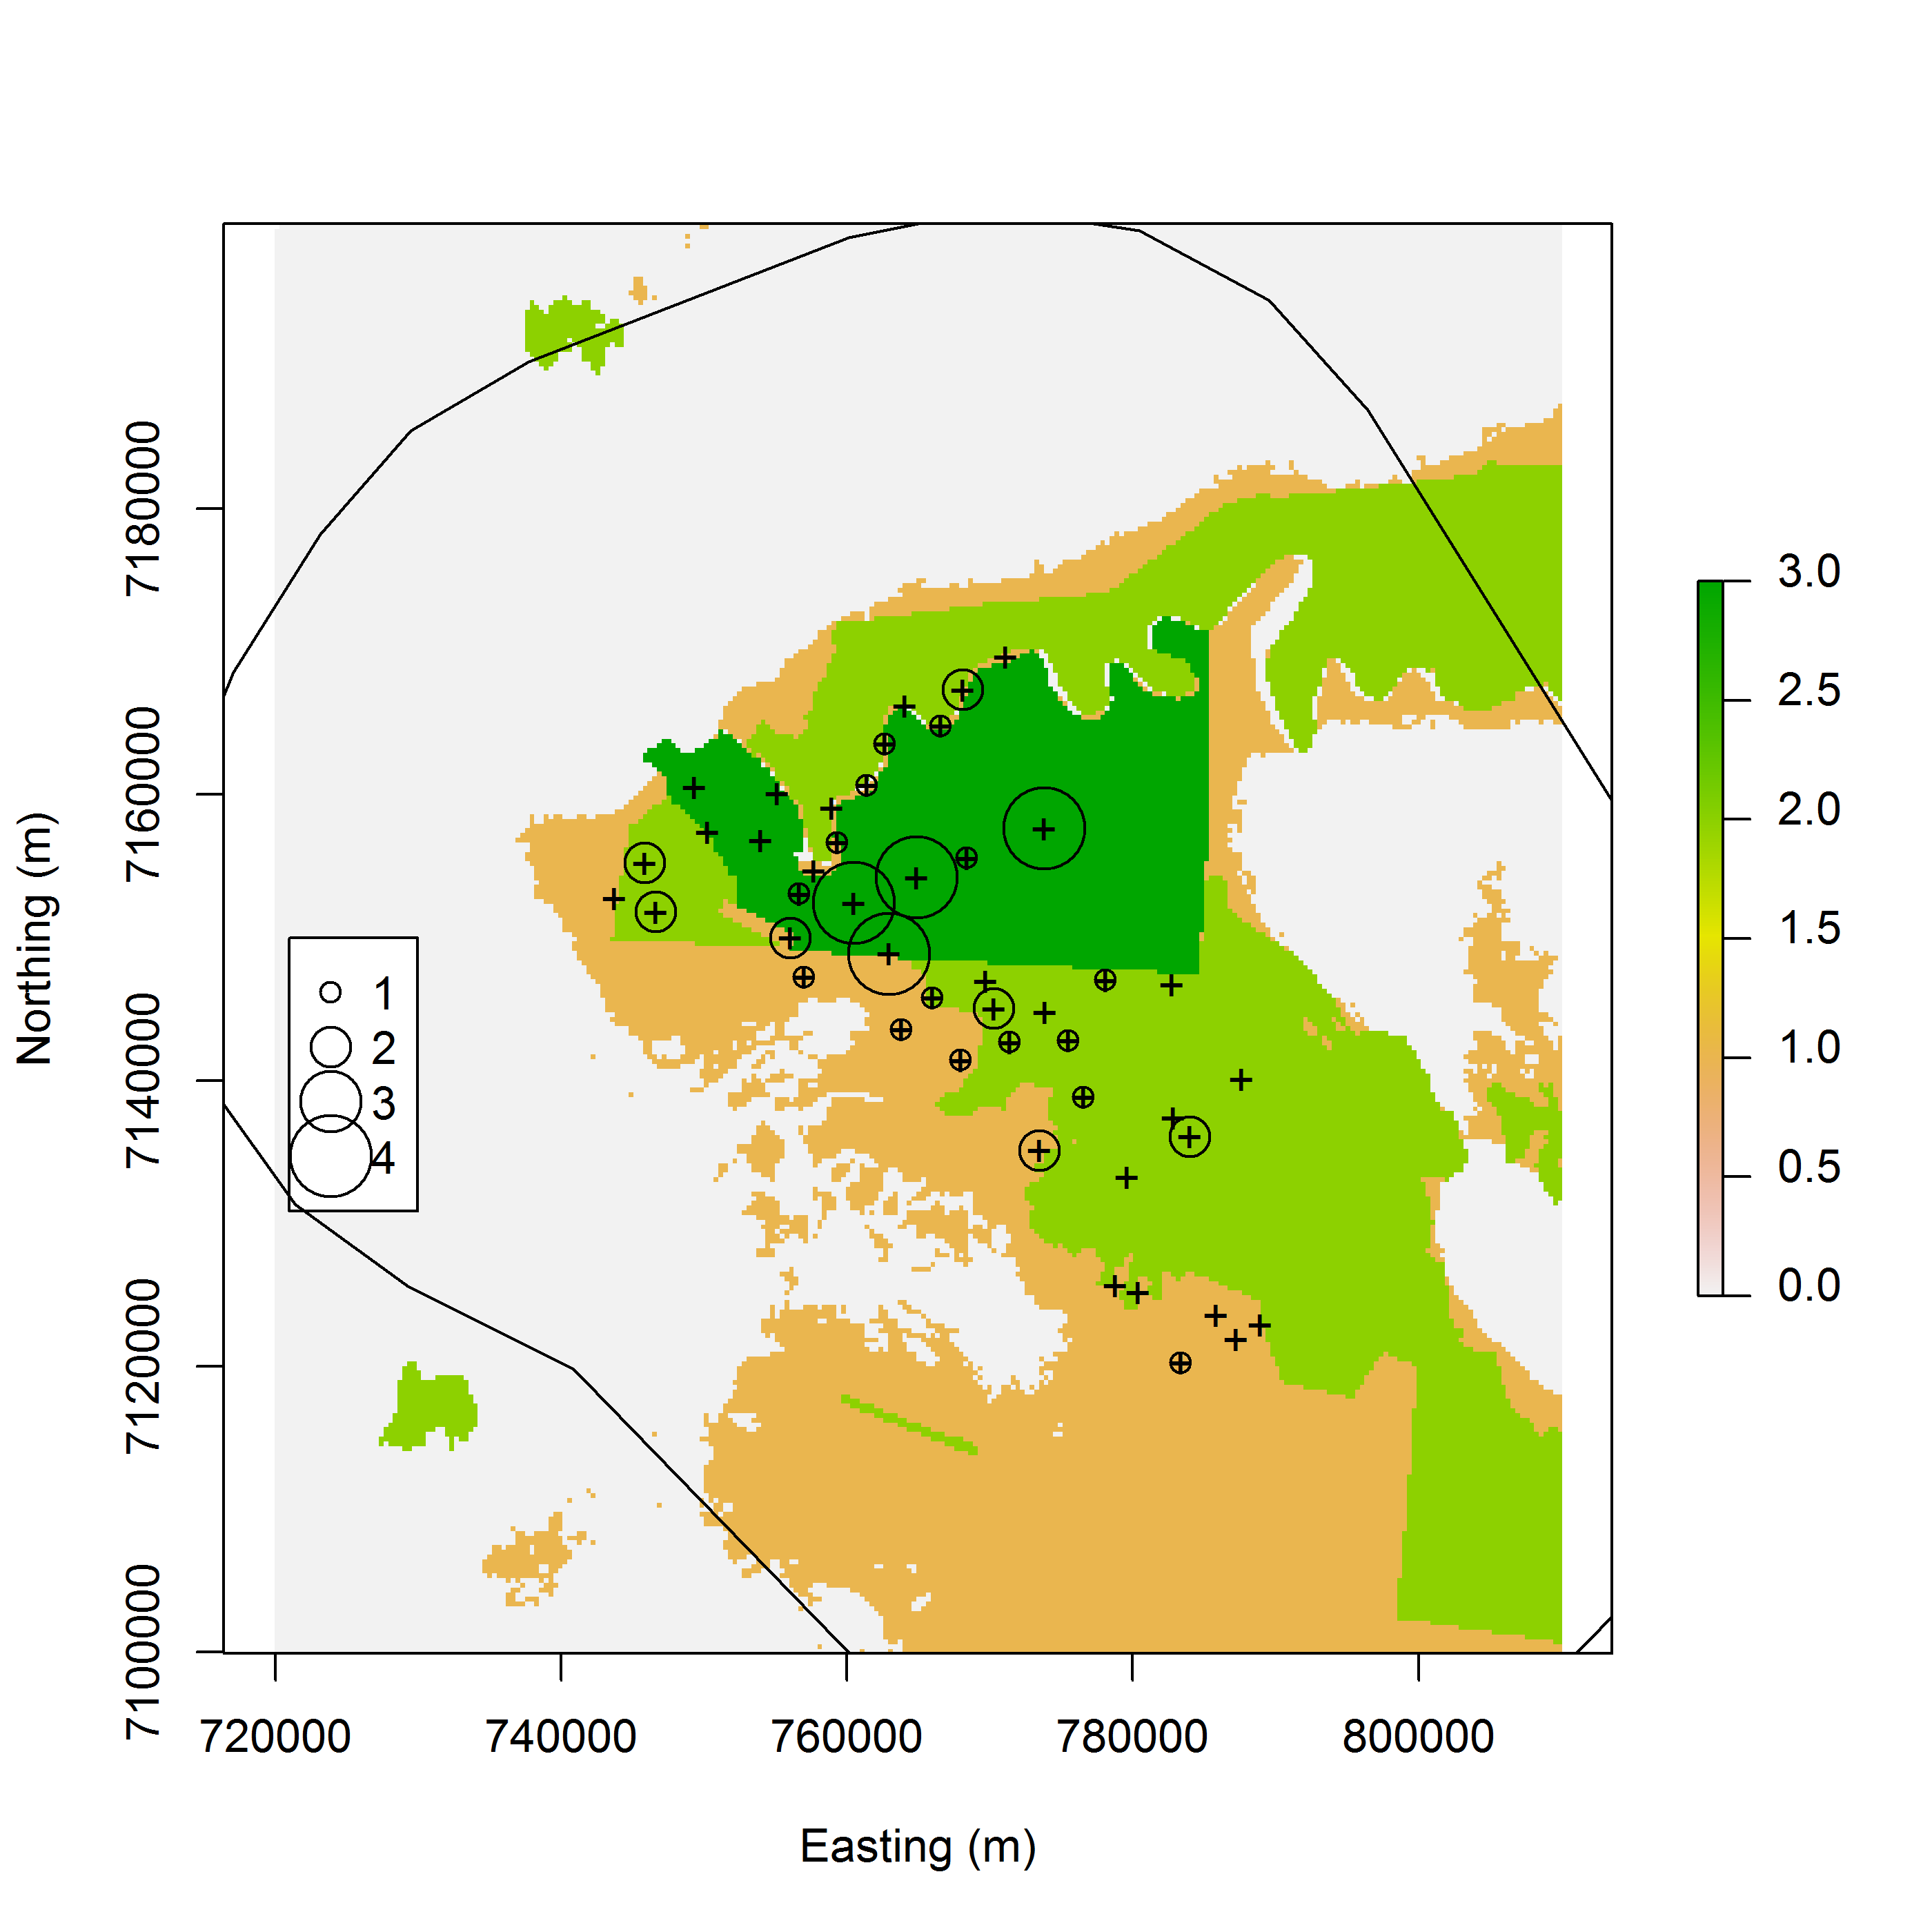
\includegraphics[width=3in,height=3in]{Ch11/figs/jaguarCountMap}
\label{ch9.fig.jaguarCts}
\caption{Jaguar detections at 46 camera trap stations. The three levels of
  protection status are no protection (beige), some protection (light
  green), and national park (dark green). Non-habitat is shown in gray
  and represents large soybean monocultures. }
\end{figure}

To assess the influence of poaching on jaguar density, we treated
protection status as an ordinal variable with 3 levels: no protection,
some protection, and high protection (national parks). Clearly these
are ordered, and our
hypothesis is that poaching pressure should decrease and jaguar
density should increase with the level of
protection. Thus, $\beta$ in this example is a ``slope''
parameter describing the degree to which protection status affects
jaguar density. We also hypothesized that males and females could have
different home range sizes and that the sex ratio may not be
1:1. Furthermore, we restricted the state-space to exclude the large
soybean monocultures surrounding the study area, and we only
considered
area south of the Iguazu River, which runs along the northern border
of the park shown in dark green in
Fig.~\ref{ch9.fig.jaguarCts}. Rather than restricting the
state-space, we could have modeled the permeability of the river using
the methods described in the previous section and in
Chapter~\ref{chapt.ecoldist}; however, no sampling was conducted on
the northern side of the river, and ancillary data indicates that
jaguars very rarely forge the waterway. \R~code to fit the model is
available in \scrbook  on the help page \verb+jaguarDataCh9+. Parameter
estimates are shown in Table\ref{ch9.tab.jagposts}.
\begin{table}
\centering
\caption{Summaries of posterior distributions from the model of jaguar
  density. $\sigma_f$ and $\sigma_m$ are the scale parameters of
  the half-normal detection function for females and males
  respectively. $\rho$ is the
  sex-ratio. $\lambda_0$ is base-line encounter rate. $\beta$ is the
  effect of protection on jaguar density. D is the overall density
  estimate. D1, D2, and D3 are the density estimates
  (jaguars/100km$^2$) for the three levels of protection. }
\begin{tabular}{lrrrrr}
\hline
& Mean & SD & 2.5\% & 50\% & 97.5\% \\
\hline
 $\sigma_f$ &  7361.731 &  1907.566 &  4899.740 &  7002.770 & 12083.110 \\
 $\sigma_m$ &  8177.068 &  1545.717 &  5916.151 &  7955.788 & 11842.486 \\
 $\rho$ &     0.516 &     0.118 &     0.286 &     0.516 &     0.741 \\
 $\lambda_0$ &     0.007 &     0.002 &     0.003 &     0.007 &     0.012 \\
 $\beta$ &     4.405 &     1.443 &     2.553 &     4.143 &     7.775 \\
 D &     0.533 &     0.708 &     0.000 &     0.000 &     0.072 \\
 D1 &     0.132 &     0.010 &     0.095 &     0.095 &     0.616 \\
 D2 &     1.415 &     0.050 &     0.214 &     0.531 &     1.503 \\
 D3 &     3.516 &     0.000 &     0.292 &     3.105 &     4.220 \\
\hline
\end{tabular}
\label{ch9.tab.jagposts}
\end{table}

Our results
indicate that efforts to protect jaguars by reducing poaching are
working. Density was $>$26 times higher in the national park than in the
unprotected area. Fig.~\ref{ch9:fig:Dsurface} shows the estimated
density surface.

\begin{figure}
\centering
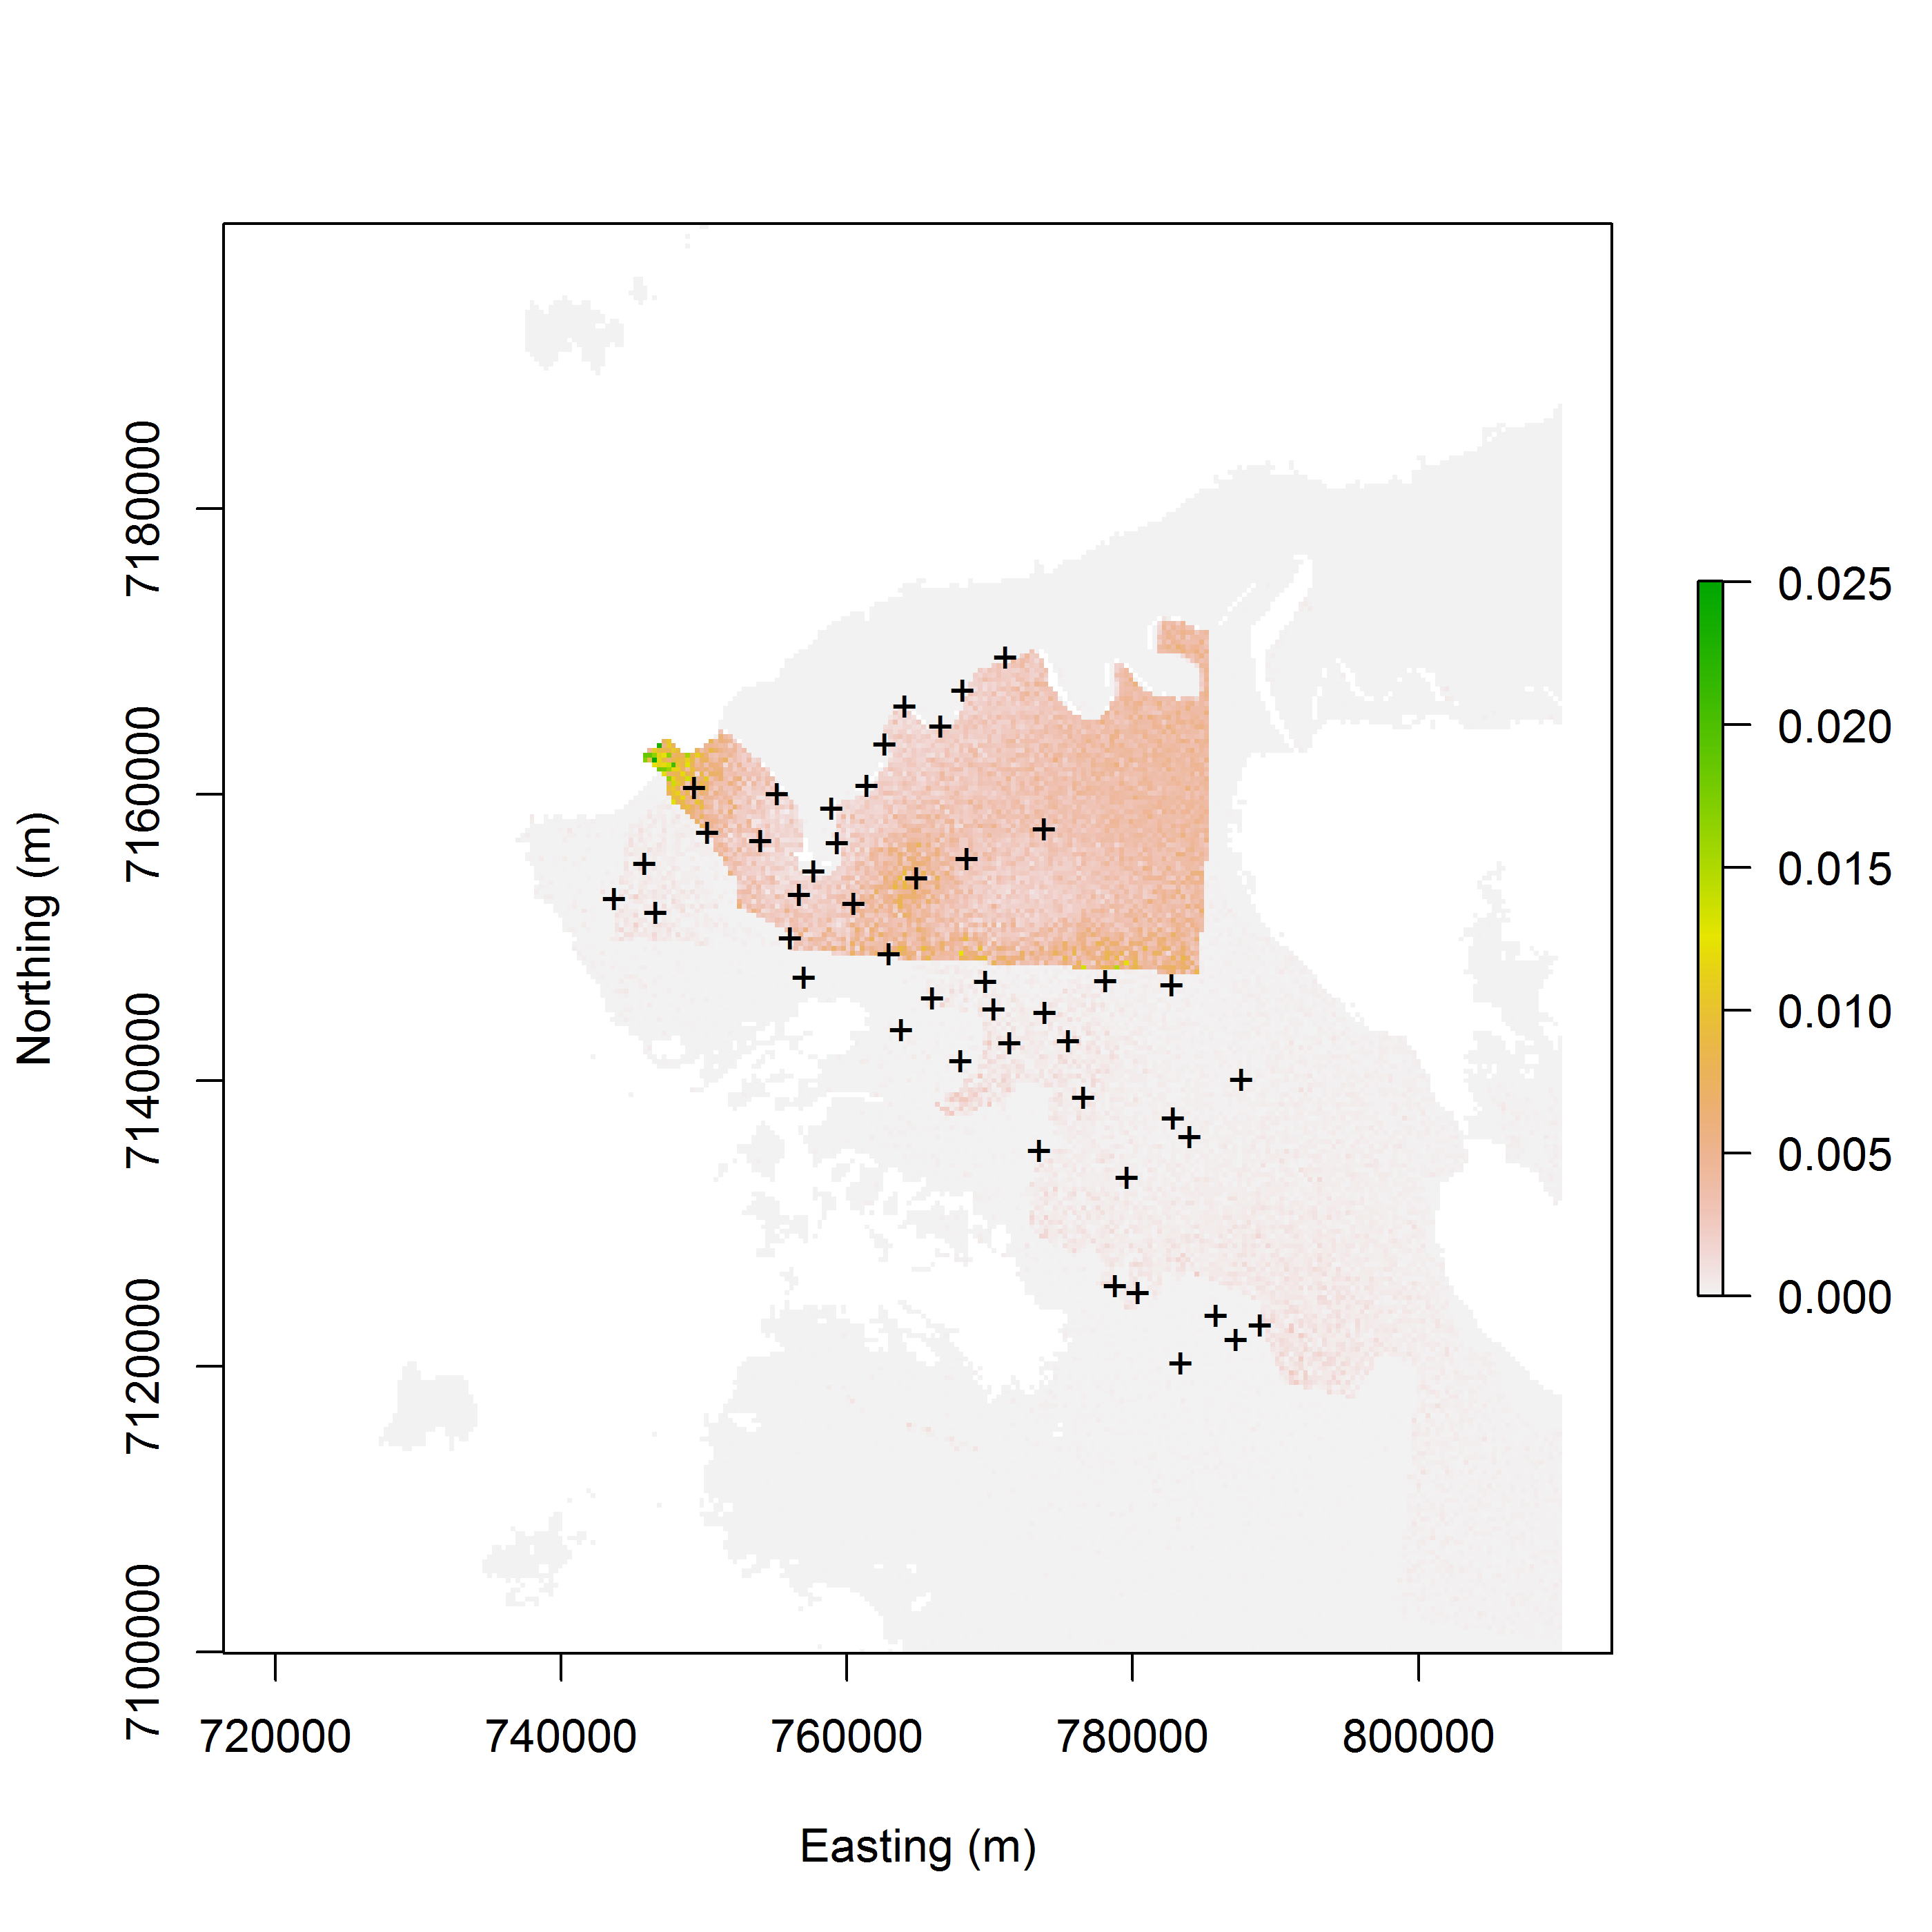
\includegraphics[width=3in,height=3in]{Ch11/figs/Dsurface34}
\label{ch9:fig:Dsurface}
\caption{Estimated density surface for the jaguar dataset}
\end{figure}


We note that there is room for improvement in our analysis. The
political boundaries used to demarcate protected areas are not as
concrete as we might like. In reality poaching pressure is likely to
be higher near remote park boundaries than in well-guarded park
interiors. One option
for addressing this would be to use a continuous measure of poaching
pressure such as distance from the nearest town, or some other
accessibility metric. It would also be interesting to model density
separately for each sex. Many of the detections outside of the park
were of males, and thus it is possible that the sexes use habitat
differently. Developing models for these two hypotheses could be
readily accomplished using slight modifications of the code found in
the \R~package \scrbook.



\section{Summary}

When state-space covariates are available,
density can be modeled by replacing the uniform prior on the activity
centers with a
prior based on a normalized log-linear function of covariates. This
distribution has been widely used in ecology to model point processes
as well as resource selection probability functions
\citep{manly_etal:2002,lele_keim:2006}. In the SCR
context, use of this new prior results in
a model for the inhomogeneous point process describing the
location of activity centers, which can be used to test hypotheses
about spatial variation in density. In
rare cases, these covariates are truly continuous in the sense that
they are defined as a function of space. More often, covariates are
represented as rasters, which simplifies the analysis. Fitting these
models can be accomplished using \bugs, \secr, or the custom \R~code
presented in this chapter and found in the package \scrbook.
%However,
%at the time this book was written, \scrbook is only software available
%for fitting models with covariates of both density and ecological
%distance.

All the examples in this section included a single state-space
covariate, but this was for simplicity only. Including multiple
covariates poses no additional challenges. Similarly, additional model
structure such sex-specific encounter rate parameters or behavioral
responses can be accommodated. Even more remarkable is the ability to
consider covariates that affect both density and ecological
distance. The ramifications of this are enormous for applied
ecological research and conservation efforts because, for instance,
researchers can use capture-recapture data to identify areas where
density is high, and to model important quantities such as landscape
connectivity \citep{royle_etal:2012ecol}. Addressing such questions
is simply not possible using standard, non-spatial capture-recapture
methods. Accomplishing these goals will of course require more data
than is needed to estimate the parameters of a basic SCR model.

